\section{Results and Discussion}

In this section, we report the findings of our user study that compare the proposed MindMargin interface against the traditional vertical commenting system. Overall, we observed a decrease in polarized views among readers who had seen or read the article previously and an increase in opinion polarization among unfamiliar readers. We also found an increase in readers' positive impressions of comments when using MindMargin. We were able to accept both of our hypotheses.

\subsection{Hypothesis 1}
Our first hypothesis predicted an increase in personal reflection when using MindMargin. Exposure to a range of diverse and controversial comments should result in the rethinking and revising of one’s own opinions. All participants were asked their stance, from Strongly For TFA to Strongly Against TFA, on a Likert scale. Using data from participants who reported to have read the comments (see above), we computed the percentage of participants who claimed a strong stance on the article. Of those assigned to the MindMargin interface, only 16\% reported to be either Strongly For TFA or Strongly Against TFA. In contrast, 26\% of the participants using the traditional commenting system reported either extreme stance. The distribution of the Likert values is also normal for MindMargin and a U-shaped curve for the traditional commenting system. We performed a Shapiro-Wilk normality test ($alpha=0.05$) on both distributions. MindMargin rejects the null-hypothesis with $p=0.1306$ and therefore is normally distributed. The traditional prototype accepts the null-hypothesis with $p=0.0205$ and is therefore not normally distributed. We created Normal Q-Q plots for both (figures \ref{fig:mm_normal} and \ref{fig:reg_normal}).

This reveals that despite no increase in the rate of reading comments, the MindMargin interface was able to encourage users to consider other opinions and viewpoints. This suggests a greater user engagement with the comments with the MindMargin interface. Therefore, we have \textbf{accepted Hypothesis 1}.
\marginpar{
\begin{figure}
  \begin{center}
  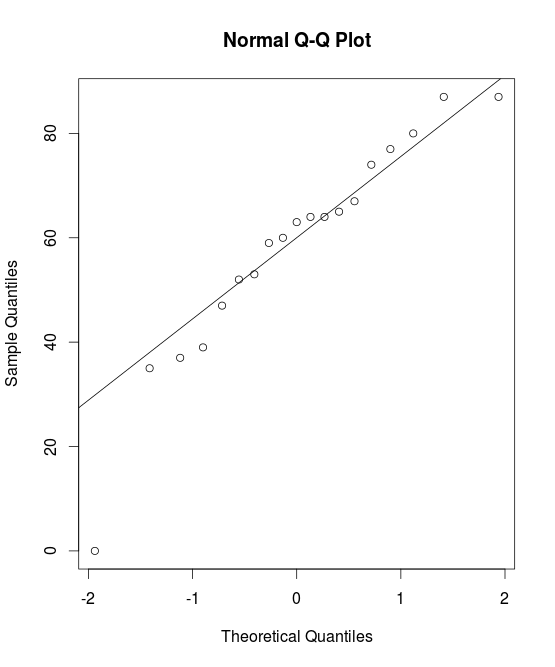
\includegraphics[width=\marginparwidth]{mm_normal.png}
  \caption{The personal stance distribution for MindMargin participants (normally distributed according to the Shapiro-Wilk normality test with $alpha=0.05$, $p=0.1306$).}
  \label{fig:mm_normal}
  \end{center}
\end{figure}
}

\marginpar{
\begin{figure}
  \begin{center}
  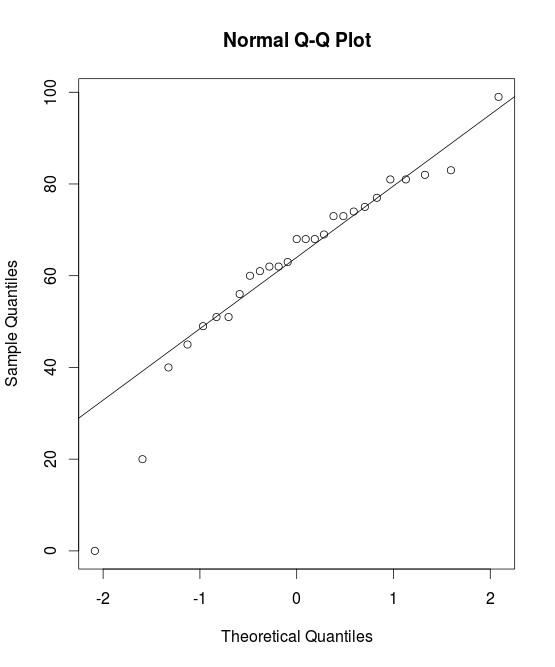
\includegraphics[width=\marginparwidth]{regular_normal.png}
  \caption{The personal stance distribution for traditional interface participants (normally distributed according to the Shapiro-Wilk normality test with $alpha=0.05$, $p=0.0205$).}
  \label{fig:reg_normal}
  \end{center}
\end{figure}
}

\subsection{Hypothesis 2}
Our third hypothesis predicted an overall increase in positive impressions on comments when using the MindMargin interface. We asked participants who read the comments to input two adjectives in free-text describing either their reaction to the comments or a description of the comments. We then classified these adjectives using a three-bin classifier (“Positive,” “Negative,” and “Neutral”). “Positive” was assigned to positive reactions to comments, such as “interesting,” “well thought-out,” and “engaging.” “Negative” was assigned to negative reactions to comments, such as “annoying,” “useless,” “distracting.” “Neutral” was assigned to descriptive input about the comments, such as “long” and “subjective.” Finally, a few outliers, such as “trolls” and “whatever,” were removed. 

We observed a drastic change of impressions when using MindMargin. As seen in figure \ref{fig:trad_pie}, the majority of participants using the traditional commenting system described the comments as negative (68\%). In contrast, when using MindMargin, the majority of participants described the comments as positive (48\%) or neutral (48\%) as seen in figure \ref{fig:mm_pie}.  Outliers were also observed only to occur in the traditional commenting system. We have therefore \textbf{accepted Hypothesis~2}. 

\marginpar{
\begin{figure}
  \begin{center}
  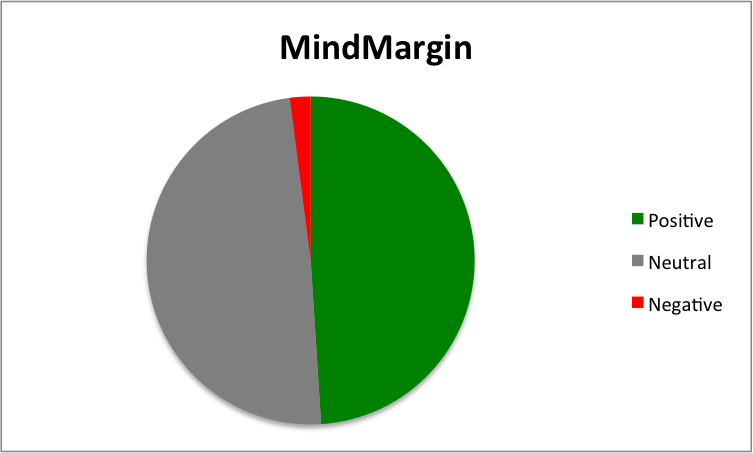
\includegraphics[width=\marginparwidth]{mm_piechart.png}
  \caption{When using MindMargin, the majority of participants described the comments as positive.}
  \label{fig:mm_pie}
  \end{center}
\end{figure}
}

\marginpar{
\begin{figure}
  \begin{center}
  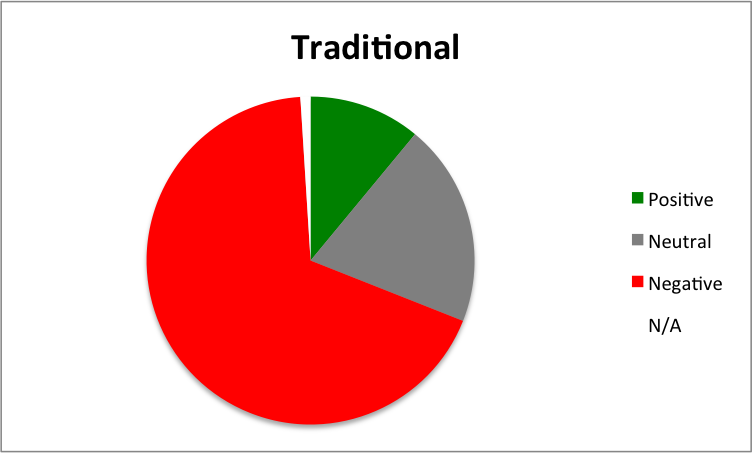
\includegraphics[width=\marginparwidth]{traditional_piechart.png}
  \caption{The majority of participants using the traditional commenting system described the comments as negative.}
  \label{fig:trad_pie}
  \end{center}
\end{figure}
}

In addition our quantitative results, we would like to quote qualitative feedback from a MindMargin user, suggesting actions he/she took beyond the scope of reading and commenting article: “This article showed me a new perspective on TFA, which after doing research, I have realized I agree with.” No feedback suggesting actions outside the scope of the article was received from participants with the traditional commenting system. 